\chapter{Data Processing}\label{ch:2}
\epigraph{On two occasions I have been asked, ""'Pray, Mr. Babbage, if you put into the machine wrong figures, will the right answers come out?'"" ... I am not able rightly to apprehend the kind of confusion of ideas that could provoke such a question.}{Charles Babbage}

The goal of data mining can be defined as the process of obtaining knowledge from underlying data by systematic using of analytic methods on it. In this thesis we are up to obtain anomalies in data and the analytic methods are the machine learning algorithms discussed in the next chapter: \ref{ch:3}. 

However, data-mining is more than applying algorithms on data. Extracting valuable results efforts among other things the consideration of a basis principle in the field of computer science known as \textit{Garbage In Garbage Out (GIGO)}. The business dictionary \footnote{http://www.businessdictionary.com/definition/garbage-in-garbage-out-GIGO.html}  defines \textit{GIGO} as an axiom used in context of computer science that signifying that no matter how sophisticated an information processing system is, the quality (accuracy, completeness, relevance, timeliness, etc) of the information coming out of it cannot be better than the quality of the information that went in. A program working on inaccurate data will only yield misleading results. The preparation of data have thus a significant contribution to the success of a data-mining goal.

There are several industry established standards like \textit{KDD, SEMMA, CRISP} \footnote{See the work of: \cite{Azevedo;Santos;Filipe:2008} for the comparison.} to name a few, invented to structure a data-mining process. The process realised in this thesis will be inclined toward to the \textit{Cross-industry process for data mining (CRISP-DM)} \cite{crisp} which is a proved data-mining process approach described in terms of an hierarchical process model.
\begin{figure}[h]
    \centering
    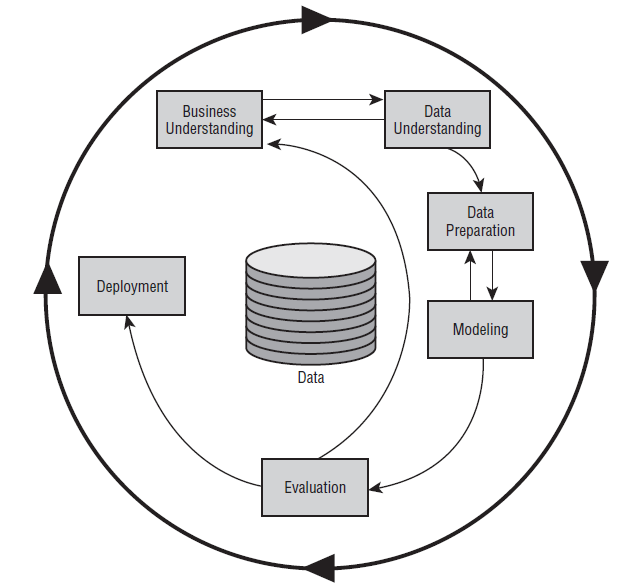
\includegraphics[scale=0.5]{Graphics/crisp-dm.png}
    \caption{CRISP-DM Process}
    \label{fig:crisp-dm}
\end{figure}
%This thesis will not adopt the complete process caused by the simple fact that a part of the methods are only for the business scope where this thesis is acting in scope of research.
\newline
\newline
\newline
This chapter will first \ref{Ch:2:Acquisition} have a macro view on the loan application process to point out the steps where our data will come from. %The goal is to have a real-world point of view on the collection process.%
Then, the first 3 phases of CHRISP-DM process are described in respect to the context of this thesis:
\begin{itemize}
    \item \textbf{Business Understanding }  
    \begin{itemize}
        \item Acquisition \ref{Ch:2:Acquisition} 
        % DATA Centered Approach, - Data driven
        \item Overview \ref{Ch:2:Overview} will discuss the macro view of the data and present insides collected by look up on it from the real-world point of view.
    \end{itemize}
    \item \textbf{Data Understanding }
        \begin{itemize}
            \item Feature Description \ref{Ch:2:FeatureDesc} provide a micro view on the available data: mention types of the features and describe the semantic.
            \item in Data Exploration \ref{Ch:2:Exploration} an  analysis of data is made by using of statistical \ref{Ch:2:SSummary} and visual \ref{Ch:2:VSummary} summary techniques, to explore data in order to bring important aspects of that data into focus. Moreover subchapter \ref{Ch:2:CorAn} expose correlated features damaging classification accuracy and data quality \ref{Ch:2:DataQuality} is dealing with inconsistent data.
        \end{itemize}
    \item \textbf{Data Preparation }
            \begin{itemize}
                \item Chapter Preprocessing \ref{Ch:2:Preprocessing} contain a composition of well researched data preparation approaches with the goal to increase the model performance. Dealing with missed/inconsistent data in \ref{Ch:2:MVI}, changing data representation to fit in the model is described in \ref{Ch:2:CTNT}. Then \ref{Ch:2:PCA} Principle Component Analysis (PCA) is applied, which is a typical statistical tool to reduce dimensions and rescale the features (give them the properties of a standard normal distribution).
        \end{itemize}
\end{itemize}

\section{Acquisition}\label{Ch:2:Acquisition}
The underlying data treated in this thesis contain information, collected during the credit enquiry process, briefly illustrated in figure \ref{fig:behav-data}. In course of the application the potential borrower provide his personal information by stepping through the application web-form. Moreover, most of the interactions with web-form elements, pressed keys or tracked time between actions is also implicitly collected. The figure \ref{fig:behav-data} show up an overview of data collecting.
The initial data used in this thesis is provided as a table. The engineering aspects regarding collecting and provisioning of the table are not part of this work and will not be discussed further. 

\begin{figure}[h]
    \centering
    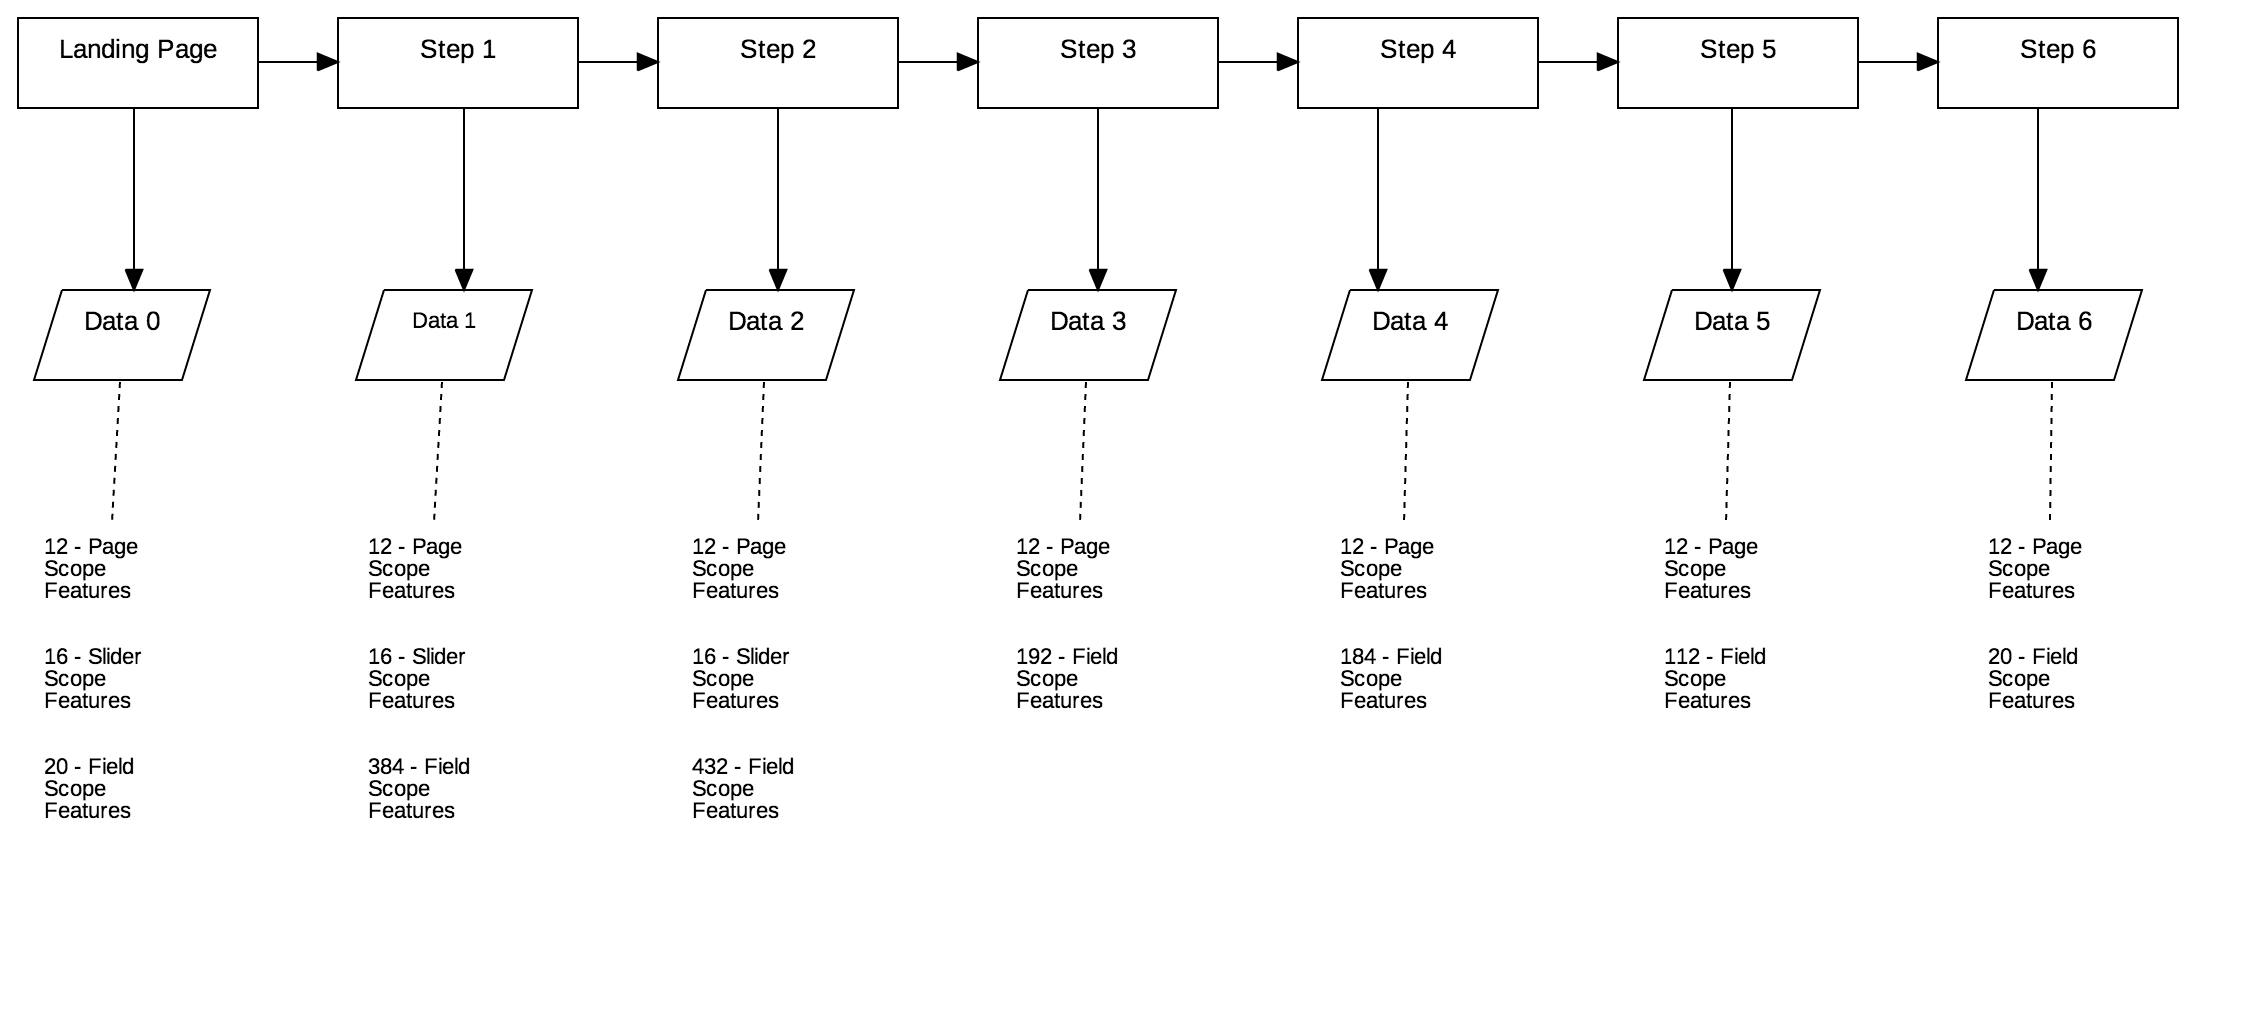
\includegraphics[scale=0.20]{Graphics/FlowchartDiagram1.png}
    \caption{Collection of Behavioral Data.}
    \label{fig:behav-data}
\end{figure}

The variables available are either categorical or numerical type and have two different sources:

\textbf{Variable Sources:}
\begin{itemize}
    \item User Input (Inputs made by the credit-applicant.)
    \item System Discovery (Variables that the application-system collect implicitly during the application-process.)
\end{itemize}

However, the variables from a scope of \textit{User Input} will be excluded from further analysis based on the fact that user inputs can be malicious. Although technical barriers are implemented, it is quite usual that fraudsters try to by-pass the process by inserting malicious information to receive a loan. This leads to the logical assumption that user generated input (such as monthly income, marital status, employee status etc.) is likely to contain intentionally false information. In comparison, the system collects continuous behavioral data \textit{Discovered by System} to detect fraudulent patterns in the course of the beginning to the end of the application process. Manipulation of behavioral information is significantly more difficult than inserting alternate personal information. The most obvious obstacle for the fraudster is to identify the technique and measures of behavioral assessment and this requires both technical experience and time which is usually not in relation to the benefits (small loan sizes). Considering these aspects, the following thesis is focusing on the behavioral data rather than the user input itself. 

\subsection{Overview (business understanding)}\label{Ch:2:Overview}

An effective utilization of data in machine learning requires a profound understanding of available data - also from a nontechnical perspective. In the following thesis, I will consider real-world aspects in which underlying data is potentially helpful for a solution.

Each data instance is representing information of an individual credit application, the information is historical and represents a common fact of a granted loan. This assortment is desirable. Granted means that this application have been approved by the scoring algorithm and the loan is issued to the borrower. Identifying anomalies signifying malicious actions in this type of data is of particular interest to prevent fraud in the future.

In following this Thesis introduce three assumptions to semantically structure (label) the available data for further algorithmic analysis.

\textbf{Fraud:} 
A small subset hold applications that in retrospect turned out to had fraudulent intention. This can have different causes, a portion has been reported by the local law enforcements, others are results of identity abuse or other malicious actions. This thesis will not amplify the fraud causes in detail and outline them simple as -  fraud.

\textbf{Non Fraud:} 
A borrower who payed at least one installment back is believed not to have any fraudulent intentions. 


\textbf{Unlabeled:}
A notable subset of underlying data contain application information not labeled as fraud but also not have positive cash flow, thus, this data can be classified as either fraud or nonfraud. 

\subsection{Feature Description}\label{Ch:2:FeatureDesc}

The underlying dataset contains in total 1804 features for each instance. All features are behavioral information which has been collected in the course of the credit application process (see: \ref{fig:behav-data}). An isolated description of each feature is not practical and thus not part of this Thesis. However, a more consolidated analysis is required. Table \ref{tab:feature-summary} summarize the data types contained in our data.


\begin{table}[h!]
  \begin{center}
    \caption{Feature type summary}
    \label{tab:feature-summary}
    \begin{tabular}{c|c|c}
    Type & Amount & Rate \\
      \hline
     Categorical & 196 & ~11\% \\ 
     \hline
     Logical & 90 &  ~5\% \\
     \hline
     Numeric & 1519 &  ~84\% \\
     \hline
    \end{tabular}
  \end{center}
\end{table}

Regarding to the figure \ref{fig:behav-data} there are 3 different scopes of behavioural features.

\begin{itemize}
    %write page on step chart
    \item \textbf{Page Scope:} Variables describing behavior in the scope of one of the 7 pages must be passed in credit application process. 
    \item \textbf{Slider Scope: } Variables in scope of an web-form element called \textit{slider}, it representing two interactive bars responsible for the adjusting of the loan amount the borrower apply for and the duration till the first installment.
    % rename to element scope
    \item \textbf{Field Scope:} Is the scope of all web form elements available through the enquiry process (input fields, buttons, check boxes, etc.).
\end{itemize}

Numerical features dominate the type distribution, in particular, most of them contain behavioral information e.g (count of keys been pressed by the user, time between interactions at input fields, etc.). Categorical features represent the types of web form elements triggered by user e.g (input field with text, drop down box with numbers, etc.). The remaining portion of logical fields containing boolean information (TRUE/FALSE) on questions regarding the behavior during the application e.g (did the user read the terms of the agreement?, did the user submitted his real email address on the first try? ... , etc.).

\section{Exploration}\label{Ch:2:Exploration}

This task addresses data mining questions using querying, visualization, and reporting techniques. These include distribution of key attributes (for example, the target attribute of a prediction task) relationships between pairs or small numbers of attributes, results of simple aggregations, properties of significant subpopulations, and simple statistical analyses. These analyses may directly address the data mining goals, they may also contribute to or refine the data description and quality reports, and feed into the transformation and other data preparation steps needed for further analysis \cite{crisp}.

\subsection{Statistical Summary of Data}\label{Ch:2:SSummary}

In total, our underlying data-set holds 95951 instances of individual applications.

According to the semantic labeling \ref{Ch:2:Overview} Table \ref{tab:instance-summary} summarize the amount of particular labels.

\begin{table}[h!]
  \begin{center}
    \caption{Instance Type Summary}
    \label{tab:instance-summary}
    \begin{tabular}{c|c|c}
    Label & Amount & Rate \\
      \hline
     Fraud & 744 & ~1\% \\ 
     \hline
     Nonfraud & 82525 &  ~86\% \\
     \hline
     Unlabeled & 12682 &  ~13\% \\
     \hline
    \end{tabular}
  \end{center}
\end{table}
It shows up that non-fraudulent instances clearly dominating the class membership where in the contrary the fraudulent representing a small subset. However, anomalies are rare by definition so this is a common pattern.

Summarizing over the category amount in categorical type features show up: 
\begin{itemize}
    \item \textbf{Min: } 2 Categories
    \item \textbf{Max: } 6 Categories
    \item \textbf{Mean:} 3 Categories
\end{itemize}
This observation is important insofar as each category adds a further dimension during the categorical to numerical transformation process \ref{Ch:2:CTNT}.
There are numerous well-known exploration techniques (like mathematical average, standard deviation or variance to name a few), unfortunately applying these on the high amount of features available would not necessary yield a valuable result. Based on this fact, further summary techniques are beyond the scopes and will not be considered.
\subsection{Visual Summary of Data}\label{Ch:2:VSummary} 
 
- Here  1-2 histograms of interesting variables, then explain that the complexity to show up everything is to high.

\subsection{Data Quality (missing values)}\label{Ch:2:DataQuality}
\epigraph{The only really good solution to the missing data problem is not to have any. Statistical adjustments can never make up for sloppy research. }{Paul D. Allison, 2001}
\label{intro}

Lack of information or missing data in a given data set is a common obstacle in field statistics and data mining. Investigations on the quality of data aim to identify lacks, which will benefit the desired machine learning algorithm. 

Bellow an descriptive analysis is made to identify the amount of missing data. Table \ref{tab:missings-over-all} present a statistical summary of missing rate in our source data.
 \begin{table}[h!]
  \begin{center}
    \caption{Summary of missing over the entire data.}
    \label{tab:missings-over-all}
    \begin{tabular}{c|c|c|c|c|c}
    Min & 1st Quartile & Max & Median & Mean & 3rd Quartile \\
      \hline
     0\% & 8\% & 99\% & 31\% & 43\% & 77\% \\ 
     \hline 
    \end{tabular}
  \end{center}
\end{table}

Since the lack of data is present, a deeper investigation is required. Missing data can have different types (in the context of statistical analysis). According to \cite{Allison:2007} there are three categories of missing data:

 \begin{itemize}
    \item \textbf{Missing Completely At Random (MCAR)} means that the probability of missing is unrelated to the variable itself or other variables. 
    \item \textbf{Missing At Random (MAR)} address missing in variables that is unrelated to itself. For example the probability of missing in income may depends on the employment status, but not depend on the income.
    \item \textbf{Not Missing At Random (NMAR)} eventuates when MAR is gone to be violated, ergo the probability of the missing depend on the particular value.
 \end{itemize}
 
Identifying the right category is important to select the correct treatment. However, classify the category of missing is not straight forward. An assumption about the membership is always based on observations on data and domain specific knowledge of data collection process.

Bellow missing amount is broken down to the summary on data grouped by type.

 \begin{table}[h!]
  \begin{center}
    \caption{Summary of missing over logical data.}
    \label{tab:missings-over-logical}
    \begin{tabular}{c|c|c|c|c|c}
    Min & 1st Quartile & Max & Median & Mean & 3rd Quartile \\
      \hline
     5\% & 9\% & 99\% & 31\% & 43\% & 76\% \\ 
     \hline 
    \end{tabular}
  \end{center}
\end{table}
 
 \begin{table}[h!]
  \begin{center}
    \caption{Summary of missing over numeric data.}
    \label{tab:missings-over-numeric}
    \begin{tabular}{c|c|c|c|c|c}
    Min & 1st Quartile & Max & Median & Mean & 3rd Quartile \\
      \hline
     0\% & 8\% & 99\% & 30\% & 41\% & 76\% \\ 
     \hline 
    \end{tabular}
  \end{center}
\end{table}
   

 \begin{table}[h!]
  \begin{center}
    \caption{Summary of missing over categorical data.}
    \label{tab:missings-over-categorical}
    \begin{tabular}{c|c|c|c|c|c}
    Min & 1st Quartile & Max & Median & Mean & 3rd Quartile \\
      \hline
     0\% & 24\% & 99\% & 59\% & 58\% & 90\% \\ 
     \hline 
    \end{tabular}
  \end{center}
\end{table}


Analytics done on missing amount of numerical \ref{tab:missings-over-numeric}, logical \ref{tab:missings-over-logical} and categorical \ref{tab:missings-over-categorical} types, show up that no type is gapless of lacks. The statistics over missings in logical and numeric data are quite similar, this fact can lead to the assumption that the causes of lacks can be related to a common factor(s). This, in turn, is indicative to MAR category of missing.

A common technique to build an assumption about the category of missing is to inspect so called \textit{missing patterns}. It contributes to understanding whether groups of variables tend to be either all missing or all observed. Table \ref{tab:variable-pattern-example} present a matrix, in which each row corresponds to a missing data pattern \textit{(1=observed, 0=missing).} 

\begin{table}[h!]
\centering
\caption{Missing pattern applied on four random variables.}
\label{tab:variable-pattern-example}
\begin{tabular}{lllll}
\textbf{Amount} & V1 & V2 & V3 & V4 \\
901             & 1           & 1           & 1           & 1           \\
20              & 1           & 1           & 0           & 1           \\
4510            & 1           & 1           & 1           & 0           \\
2               & 0           & 1           & 1           & 1           \\
6               & 1           & 0           & 1           & 1           \\
87847           & 1           & 1           & 0           & 0           \\
9               & 0           & 1           & 1           & 0           \\
55              & 1           & 0           & 0           & 1           \\
6               & 1           & 0           & 1           & 0           \\
572             & 0           & 1           & 0           & 0           \\
716             & 1           & 0           & 0           & 0           \\
1307            & 0           & 0           & 0           & 0          
\end{tabular}
\end{table}

Furthermore, there is a visual investigation approach to identify missing patterns. Figure \ref{fig:missing-plot} present two plots. The histogram shows up the rate of missing values and the box plot is the visualisation of missing patterns.

\begin{figure}[h!]
    \centering
    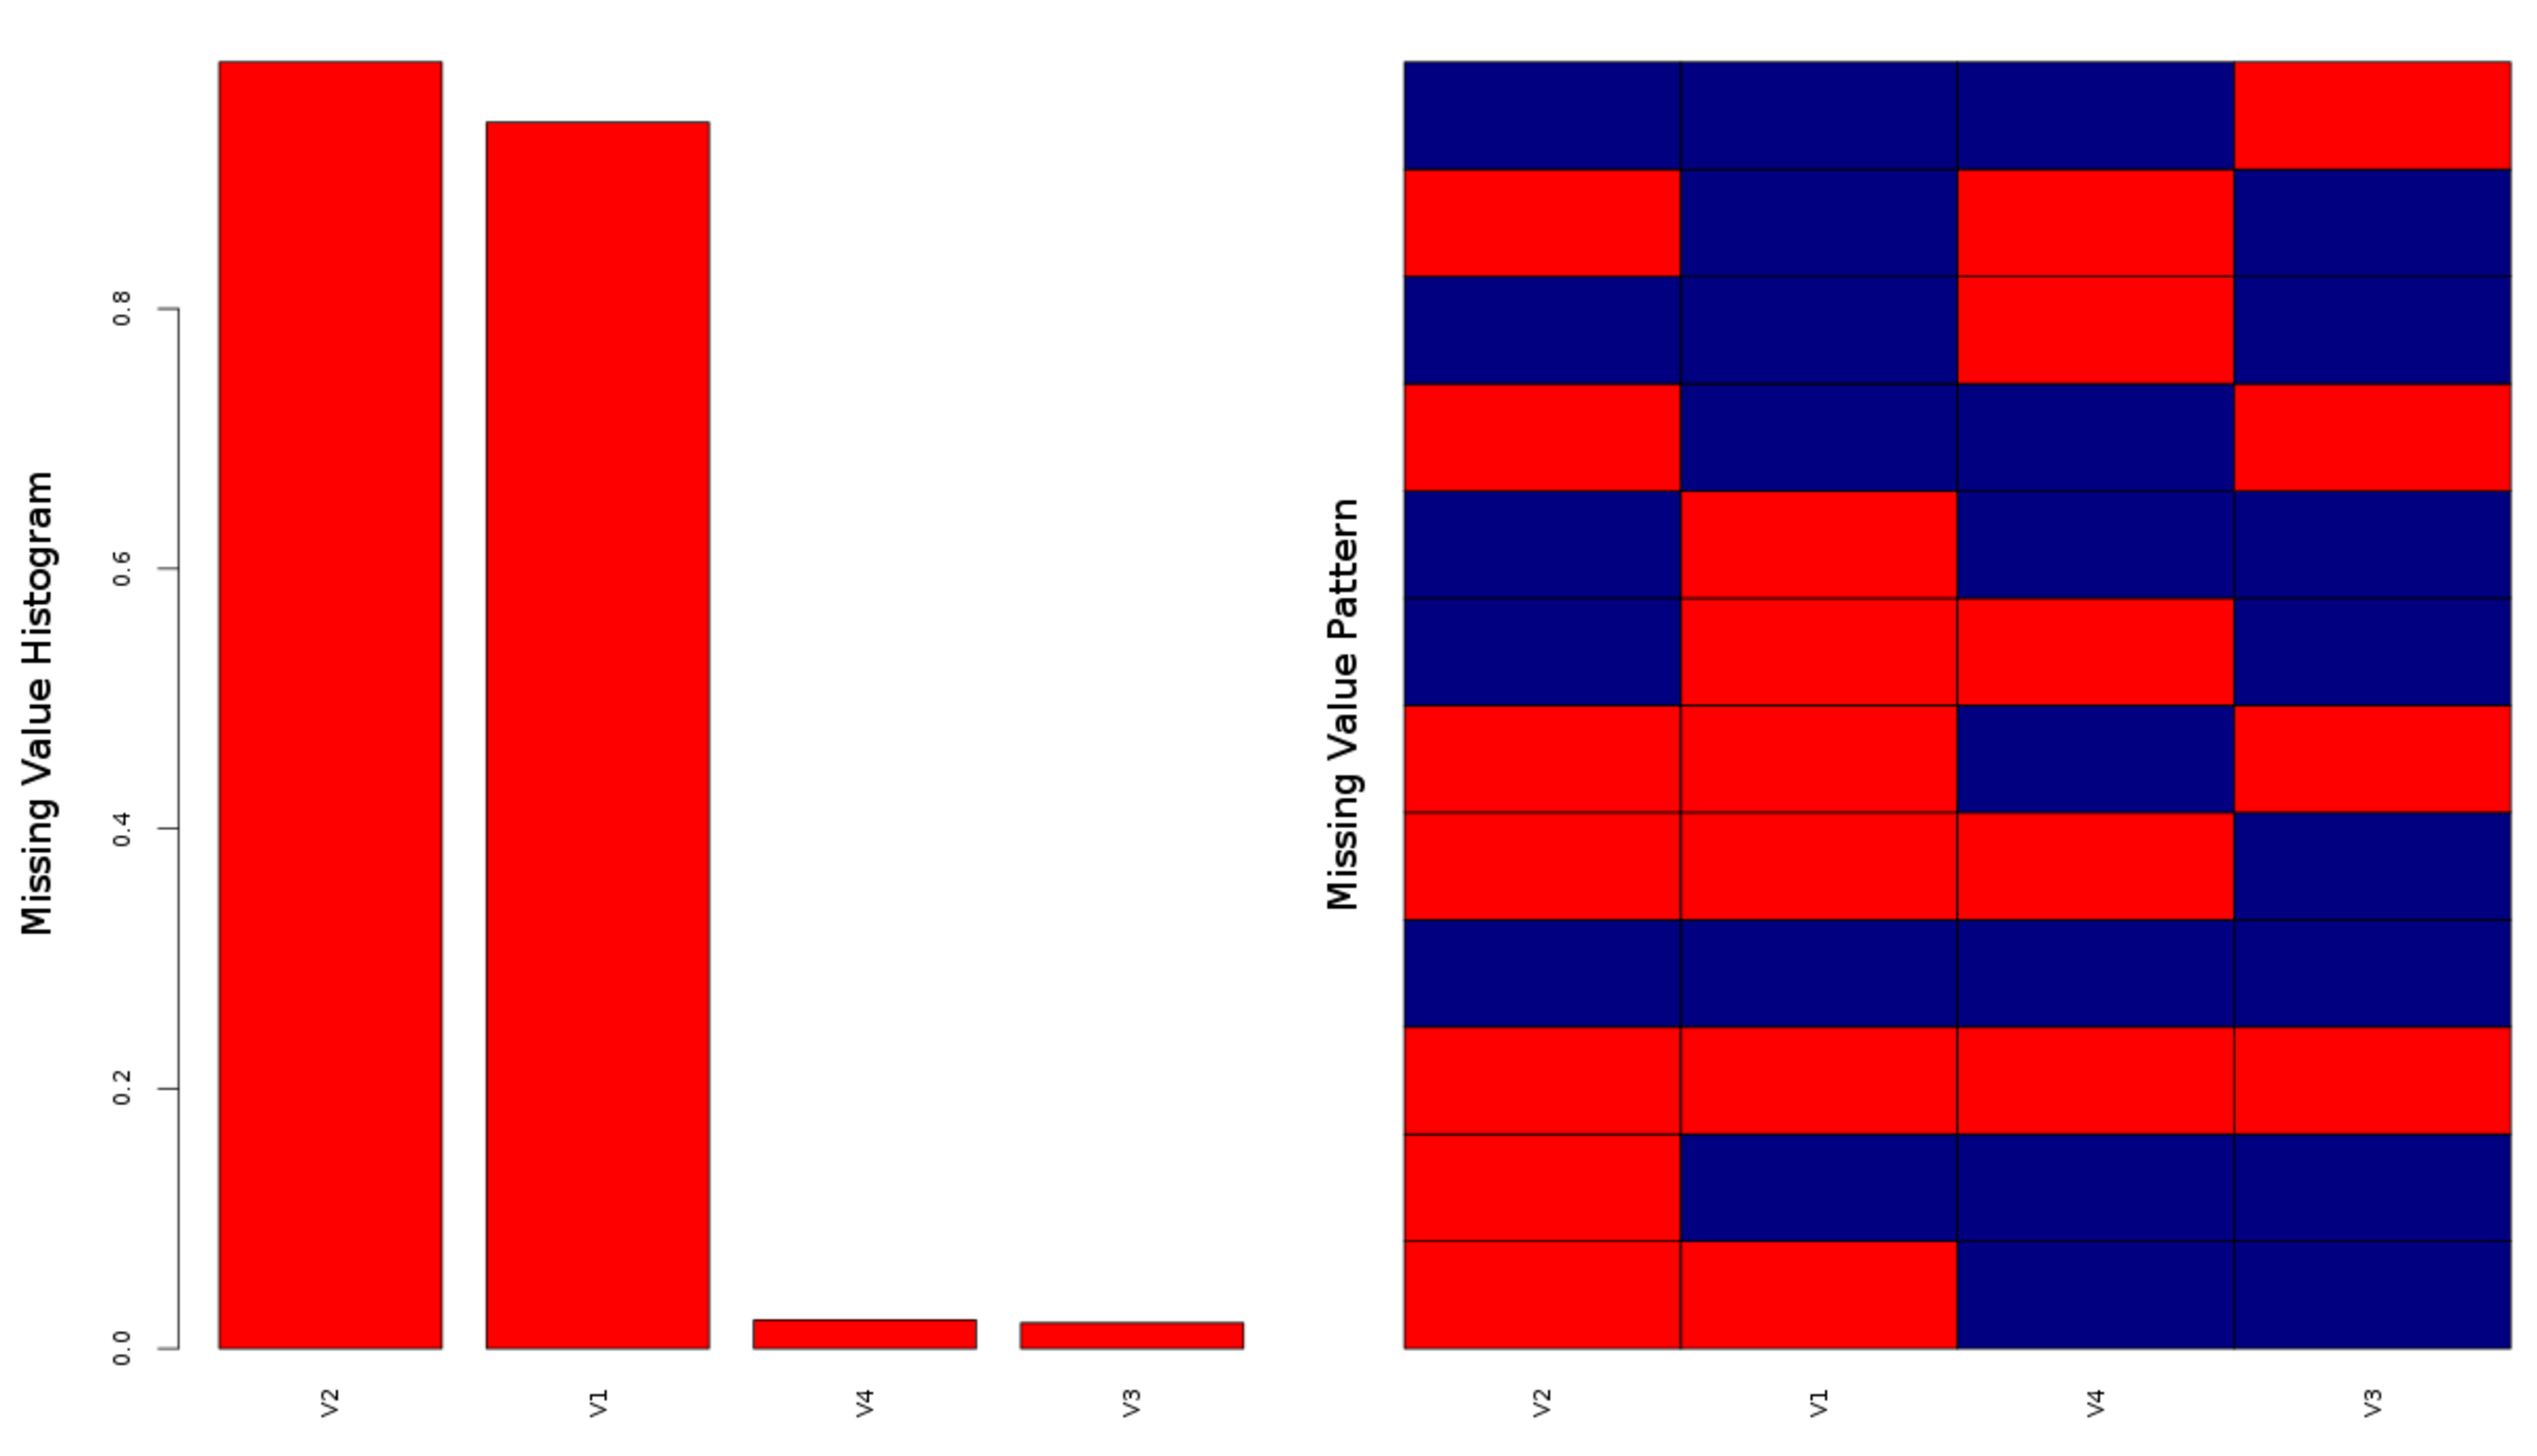
\includegraphics[scale=0.3]{Graphics/missing-pattern-plot.png}
    \caption{Plot possible patterns of missing data.}
    \label{fig:missing-plot}
\end{figure}

Unfortunately, these methods of analysis not fitting well with our amount of features. A pattern matrix describing all possible patterns on data given in this thesis would be obviously hard to manage. Pattern analysis can also be applied to a subset of data - to yield more coherent results, However, the creation of the suitable subset efforts an assumption to chose the suspicious features.

It is conceivable, that more advanced analytics would produce valuable results in the case of missingness classification. However, this topic would deserve a separate research paper and exceed the scope of this thesis. Furthermore, the interested reader is referred to the work of \cite{Mohan;Pearl:2014} where a promising approach for Testability of missing category is provided.

As last but not least, initial improving data quality should also be considered. Possible causes of missing values can be a helpful information to start with quality treatment. 
Potential causes could be:
    \begin{itemize}
    
        \item Behavior data is describing several interactions with web form components, some of them are optional.
        
        \item Application data is obviously processed through several instances before it is available for data analysis. The processing and data conversions related to this process could be responsible for the loss of data.
        
        \item The credit application process was executed by a non-human but so-called script/bot \footnote{A bot (short for "robot") is a program that operates as an agent for a user or another program or simulates a human activity on the Internet. (http://searchsoa.techtarget.com/definition/bot)}. A bot obviously skips the most of the interactions a human would have to do during the application. 
    
        \item The particular operation system on top the application is executed can be modified to block the gathering of information by the application system.
    \end{itemize}


\section{Preprocessing}\label{Ch:2:Preprocessing}
Based on the observations obtained through acquisition and exploration of our data, this section will explain the explicit steps of data transformation made before fitting it in our model.

\subsection{Missing Value Imputation}\label{Ch:2:MVI} 
  IN PROGRESS (To Liuben: already imputed everything as median, i will reason it with the easiest method, please leave a short note if you agree or not and why :))
 
\subsection{Categorical to Numeric Transformation}
\label{Ch:2:CTNT}
The most of the statistical learning algorithms like them provided in this thesis (chapter: \ref{ch:3}), can't deal with other than numerical data types. Since the analysis of a number of types contained in our data \ref{tab:feature-summary}, is known that beside numerical also categorical and logical types are components of given feature set. 

Thus, a number of nonnumerical features are not minor, the utilization of these can have a significant impact on model accuracy. A common approach to convert categorical values into numerical representation is binarization where each value is transformed in either 1 or 0.

Let us consider a categorical feature \textit{action} describing the input behavior happened to process the next step during the credit inquiry, the possible categories were given: 


\[ \{ButtonClick, MouseClick, Other\} \]

For the sake of simplicity we consider a subset with only four instances see table \ref{tab:feature-categorical-rep} for an example representation. 

\begin{table}[h!]
  \begin{center}
    \caption{Example of categorical representation.}
    \label{tab:feature-categorical-rep}
    \begin{tabular}{c|c}
    instance & action \\
      \hline
     A & Other \\ 
     \hline 
       B & MouseClick \\ 
     \hline
       C & ButtonClick \\ 
     \hline
       D & Other \\ 
     \hline
    \end{tabular}
  \end{center}
\end{table}

Applying the binarization on these would yield three additional features with an numerical value of either \(1\) or \(0\). Table \ref{tab:feature-binarization} illustrates the view after binarization.

\begin{table}[h!]
  \begin{center}
    \caption{Example of feature binarization.}
    \label{tab:feature-binarization}
    \begin{tabular}{c|c|c|c|}
    instance & action.ButtonClick & action.MouseClick & action.Other \\
      \hline
     A & 0 & 0 & 1 \\ 
     \hline 
       B & 0 & 1 & 0 \\ 
     \hline
       C & 1 & 0 & 0 \\ 
     \hline
       D & 0 & 0 & 1 \\ 
     \hline
    \end{tabular}
  \end{center}
\end{table}

However, each possible category adds another feature ergo another dimension to the underlying data set, it should be considered that high amount of dimensions have several side effects like increasing computation time or noise.

\subsection{Removing (near) Zero Variance Features}\label{Ch:2:RNZVF}
After the quality of data is been treated its time to care about reducing model complexity. Removing of predictors with zero and near zero variance is a typical preprocessing technique used for dimension reduction. 

Observations made by inspecting the data quality \ref{Ch:2:DataQuality} showed up  a non-inconsiderable amount of missing values, this fact leads to the assumption that our underlying data could be contaminated with low and zero variance features.

\textbf{Zero variance:} stands basically for statistical variance is zero, so the predictor is a constant.

\textbf{Near zero variance:} is more complex and means to identify  variables with a low unique value rate - relative to the number of samples or have a large ratio of the most common value in respect to the second most common value.

Summarized it can be said that removing can drastically reduce the computation time and also increase model accuracy by doing dimension reduction. However, removing it is not necessary always the best way, for example, an binary feature with lots of zeroes and few ones could be an legit indicative for class membership but the near zero variance process would possibly remove it.

Another considerable aspect is that normally the historical data is growing with the time - so, the probability that the variance will change is given.

\subsection{Principle Component Analysis (PCA)}\label{Ch:2:PCA} 
Principle Component Analysis is one of the main methods to reduce dimensionality, first introduced by Karl Pearson \cite{Pearson:1901}. The main idea behind PCA is to find patterns by identifying high correlated feature and remove them - dimensionality decreasing. The leftovers are the maximal variance components that contain the most information.  

The analysis made in chapter \ref{Ch:2:FeatureDesc}, showed up a lot of features contained in the underlying dataset, moreover the transformation of categorical and logical to numerical features \ref{Ch:2:CTNT} will extend the feature size. Based on the fact of large feature space and on experiments already done combining classification algorithms and dimensionality reduction \cite{5446692}, doing PCA is a reasonable process to help improve the discriminative power of classifiers.

Formally, the goal of PCA is to produce given examples from higher to lower space:

\[ x \in X \in {\rm I\!R}^n \textrm{ to } z \in Z \in {\rm I\!R}^k \]
\[ \textrm{where } k \leq n \]

The classical approach is first to compute a \(n \times n \) covariance matrix, where each element is the covariance between two features:

\[ \Sigma = \frac{1}{m}\sum_{i = 1}^{n}(x^i)(x^i)^T\]
\[ \textrm{where }(x^i) \textit{ is an } (1 \times n) \textrm{ vector and } (x^i)^T \textrm{is an } (n \times 1) \textrm{ vector.}\]

Based on the result of the covariance matrix, eigenvectors should be computed. Eigenvectors determine the direction of new feature space and their eigenvalue explain the variance of the data.
There are several methods to figure out the eigenvectors, in this thesis \textit{Singular Value Decomposition} (SVD) will be used, which is known to be rather numerical stable than the native one method called \textit{eigendecomposition}. 

Applying SVD on the covariance matrix, yield:

\[ [U,S,V] = SVD(\Sigma)\]
\[ \textrm{where  } U \in  {\rm I\!R}^{n \times n} \textrm{ Matrix representing the eigenvectors.}  \]

Sorting eigenvalues of the given eigenvectors and choosing the \( k \) count corresponding to the largest eigenvalues, will result in \( U' \in   {\rm I\!R}^{n \times k}\) matrix.
Transforming the original data \( X \) to the projection \( Z \) by:

\[ Z = X U'^ T \]
finally makes the deal to transform initial data to k-dimensional feature subspace.

Nonetheless, dimensionality reduction is always an act of information loss, so the fact that PCA can also hurt classification accuracy should be considered. Moreover, several methods for dimensionality reduction were compared in combination with classification algorithms and showed partially better results than PCA \cite{Cao2003321}. 